% Final project report -- compile with pdfLaTeX (Overleaf default).
\documentclass[11pt,a4paper]{article}

\usepackage[T1]{fontenc}
\usepackage[utf8]{inputenc}
\usepackage{lmodern}
\usepackage{microtype}
\usepackage[a4paper,margin=2.5cm]{geometry}
\usepackage{amsmath,amssymb}
\usepackage{graphicx}
\usepackage{booktabs}
\usepackage{tabularx}
\usepackage{multirow}
\usepackage{float}
\usepackage[labelsep=period,justification=raggedright,singlelinecheck=false]{caption}
\usepackage{titlesec}
\usepackage{tocloft}
\usepackage{enumitem}
\usepackage{xcolor}
\usepackage{algorithm}
\usepackage{algpseudocode}
\usepackage[hidelinks]{hyperref}

\graphicspath{{figures/}{../docs/figures/}}
\setlength{\parindent}{0pt}
\setlength{\parskip}{0.55em}
\renewcommand{\arraystretch}{1.15}
\newcolumntype{Y}{>{\raggedright\arraybackslash}X}
\setlist{itemsep=0.15em,topsep=0.3em}

% "1. Introduction" style headings, as in the department template
\titleformat{\section}{\Large\bfseries}{\thesection.}{0.6em}{}
\titleformat{\subsection}{\normalsize\bfseries}{\thesubsection}{0.6em}{}
\titleformat{\subsubsection}{\normalsize\bfseries}{\thesubsubsection}{0.6em}{}
\titlespacing*{\section}{0pt}{1.6em}{0.8em}
\renewcommand{\cftsecaftersnum}{.}
\renewcommand{\cftsecleader}{\cftdotfill{\cftdotsep}}
\renewcommand{\contentsname}{Contents}
\captionsetup[table]{position=top,skip=4pt}

\newcommand{\prisk}{P_{\mathrm{risk}}}
\newcommand{\code}[1]{\texttt{#1}}
\newcommand{\repourl}{\url{https://github.com/Abhay0912/uncertainty-aware-load-balancer}}

\begin{document}

% ================================================================ title page
\hypersetup{pageanchor=false}
\begin{titlepage}
\centering
\vspace*{0.6cm}

\includegraphics[width=3.4cm]{nitw_logo.jpg}\par
\vspace{1.4cm}
{\large\bfseries NATIONAL INSTITUTE OF TECHNOLOGY, WARANGAL\par}
\vspace{1.0cm}
{\large\bfseries PROJECT REPORT\par}
\vspace{1.0cm}
{\LARGE\bfseries Uncertainty-Aware Load Balancing with\\[0.25em] Task Completion-Time Prediction\par}
\vspace{0.8cm}
{\large Final Report\par}
\vspace{1.0cm}
{\large Master of Technology\\[0.35em] Department of Computer Science and Engineering\par}
\vspace{1.8cm}
{\large\bfseries Submitted by\par}
\vspace{0.8cm}
{\large\bfseries Abhay Nagesh Rao\par}
{\large Roll No.: 26CSM1R01\par}
\vspace{0.6cm}
{\large\bfseries Parthajeet Deva Sarmah\par}
{\large Roll No.: 26CSM1R15\par}
\vfill
\end{titlepage}
\hypersetup{pageanchor=true}

\pagenumbering{arabic}
\setcounter{page}{1}

% ================================================================ abstract
\section*{Abstract}
\addcontentsline{toc}{section}{Abstract}
This project studies how incoming tasks should be assigned to a small cluster of heterogeneous cloud
servers. A discrete-time Python simulator models five servers that differ by a factor of sixteen in
capacity, each with CPU and memory reservations and a strict FIFO queue. Two seeded workloads with
the same mean offered load, one stable and one bursty, are given unchanged to every policy, so that
differences in outcome are attributable to placement alone.

The work proceeded in two stages. The first stage (V1) proposed an \emph{uncertainty-aware probabilistic}
policy that converts the rolling mean and variance of each server's load into an overload probability,
$\prisk = 1-(1-P_C)(1-P_M)$, and adds it to a load score. Against a matched ablation without the risk
term, it did not help: it was 0.29\,s slower on the stable workload (better on none of the 5 seeds) and
within seed noise under bursts. The risk estimate was well calibrated (0.74 predicted vs.\ 0.72 observed) but not
discriminative, because a good balancer makes all servers rise and fall together. The same stage showed
that observing \emph{queued} demand, rather than utilisation alone, is worth about two orders of magnitude
in response time.

The second stage (V2) replaced server-level risk with a task-level prediction. For each candidate server,
a shadow copy of its running tasks and FIFO queue is advanced to predict when the incoming task would
finish; the \emph{earliest completion time} (ECT) policy chooses the server with the smallest prediction.
On a matched evaluation of the first 1,000 tasks of each trace over five seeds, ECT-only gave the lowest
p95 response time on both workloads (14.21\,s stable, 67.41\,s bursty), the lowest stable SLA violation rate
(1.6\%), the highest stable throughput, and the lowest bursty mean response (30.79\,s); against the two
strongest baselines these advantages held on all five seeds. It did not give the lowest stable mean response,
where Least CPU (6.99\,s) remained best. Adding an uncertainty premium on the
predicted 90th percentile did not improve ECT on any latency or SLA measure (0 of 5 seeds).

Across both stages the conclusion is consistent: \emph{which} quantity a balancer predicts matters more than
attaching uncertainty to it. All results are simulation results under stated assumptions and are not
claims about production clouds.

\textit{Keywords: cloud computing; load balancing; task scheduling; completion-time prediction; uncertainty;
overload probability; heterogeneous servers; simulation; ablation study.}

\subsection*{Principal findings}
\begin{itemize}
  \item Load-blind placement (Round Robin, Random) is one to two orders of magnitude slower than load-aware
        placement, because it gives the smallest server a fifth of all tasks.
  \item A variance-based overload probability (V1) was calibrated but could not rank servers, and did not beat
        its own ablation at the declared parameters or anywhere in a 44-point sensitivity sweep.
  \item Task-level completion-time prediction (V2) improved tail latency and throughput over every baseline in the
        matched evaluation; an added uncertainty premium did not.
  \item Measured results are reported separately from proposed future experiments.
\end{itemize}

\clearpage
\tableofcontents
\clearpage

% ================================================================ 1
\section{Introduction}

\subsection{Background and motivation}
A load balancer decides, for every arriving request or task, which server will run it. In a cloud
cluster the servers are rarely identical: instance types, hardware generations and co-located workloads
give them different numbers of cores, amounts of memory and processing speeds. A poor decision does not
fail loudly. It places a task behind a queue, or on a slow machine, and the cost appears later as response
time and as violations of a service-level agreement (SLA). Tail latency, rather than the mean, is often
what users notice~\cite{dean2013}.

Most practical policies act on a \emph{point value} of the current state: the number of open connections,
the CPU utilisation, or a weighted mix of such metrics. This project asks whether a balancer can do better
by reasoning about what is \emph{likely to happen}. Two forms of that idea are tested. The first treats a
server's recent metrics as a random variable and estimates its probability of overload. The second
predicts, for the specific incoming task, how long it would take to finish on each server.

\subsection{Problem formulation}
The cluster has $N=5$ servers. Server $i$ has $c_i$ cores, $m_i$\,GB of memory and speed $v_i$. A task
$\tau$ arrives at tick $a_\tau$ with CPU demand $d^{C}_\tau$, memory demand $d^{M}_\tau$ and work
$w_\tau$ (seconds at speed~1). Once started on server $i$ it holds its resources for
$\lceil w_\tau / v_i \rceil$ ticks. The scheduler must choose a server $i^\star$ at arrival, using only the
information a real scheduler would have, so that the response time $R_\tau = f_\tau - a_\tau$ (finish minus
arrival, including queueing) is small and rarely exceeds $R_{\mathrm{SLA}} = 18$\,s. The actual work
$w_\tau$ is hidden from the scheduler.

\subsection{Research objectives and scope}
\begin{itemize}
  \item Build a reproducible simulator in which every policy receives identical task traces and fresh servers.
  \item Implement six conventional baselines and a matched ablation for each proposed component.
  \item Design and evaluate a probabilistic overload-risk policy (V1) under a pre-declared protocol.
  \item Design and evaluate task-level completion-time prediction with and without an uncertainty premium (V2).
  \item Report aggregate, tail and paired per-seed results, and state the limits of what they establish.
\end{itemize}
The scope is an offline, single-dispatcher simulation study. Real deployment, stale telemetry and multiple
concurrent dispatchers are discussed but not evaluated.

% ================================================================ 2
\section{Research background}

\subsection{Load-balancing policies}
\textbf{Round Robin} sends task $k$ to server $k \bmod N$; it needs no state but is blind to both capacity
and load. \textbf{Weighted Round Robin} assigns tasks in proportion to fixed weights such as capacity; the
\emph{smooth} variant used in nginx~\cite{nginx} interleaves servers so a heavy server does not receive long
consecutive runs. \textbf{Least-loaded} rules choose the server with the smallest current metric; with
stale information they herd, sending every task to the same apparently idle server. \textbf{Power of Two
Choices} samples two servers and picks the less loaded one, which reduces the maximum load from
$\Theta(\log n/\log\log n)$ to $\Theta(\log\log n)$ for $n$ balls in $n$ bins~\cite{azar1999,mitzenmacher2001}.
Join-Idle-Queue~\cite{lu2011} targets large dispatcher fleets, and cluster managers such as
Borg~\cite{verma2015} combine feasibility filtering with a scoring function, a structure both proposed
policies share.

\subsection{Uncertainty and completion-time prediction}
Cluster traces show that resource usage is heterogeneous and changes quickly~\cite{reiss2012,tirmazi2020},
which motivates using variability as well as level. Treating a metric as a random variable gives a natural
risk measure, the probability of exceeding a threshold. Probabilistic forecasts are judged by
\emph{calibration} (do predicted probabilities match observed frequencies?) and by
\emph{sharpness} (do they separate cases?)~\cite{gneiting2007}; that distinction turned out to be central to
the V1 result. Completion-time heuristics have a long history in heterogeneous computing:
\emph{minimum completion time} and its batch variants assign each task to the machine on which it is
expected to finish earliest~\cite{braun2001}. V2 applies that idea online, with a duration estimate learned
from completed tasks and an explicit model of each server's FIFO queue.

\begin{table}[H]
\caption{Methodological components and their functions.}\label{tab:components}
\begin{tabularx}{\linewidth}{lY}
\toprule
\textbf{Component} & \textbf{Role in the study}\\
\midrule
Matched seeded traces & Give every policy the same tasks, so differences come from placement\\
Load signal with queued demand & Make backlog visible to load-aware policies\\
Overload probability (V1) & Estimate each server's risk of exceeding a threshold from its recent variability\\
Duration estimator (V2) & Predict a task's work from public hints and completed tasks only\\
Shadow-queue projection (V2) & Predict when the task would start and finish on each server\\
Matched ablations & Isolate the contribution of each proposed component\\
Paired per-seed comparison & Cancel workload noise and report seeds won\\
\bottomrule
\end{tabularx}
\end{table}

% ================================================================ 3
\section{Simulation environment}

\subsection{Cluster}
Five heterogeneous servers are used (Table~\ref{tab:servers}). Capacity is measured as cores $\times$ speed.
Server~4 holds 1/37 of the total capacity, which exposes any policy that ignores capacity.

\begin{table}[H]
\caption{Server configuration.}\label{tab:servers}
\centering
\begin{tabular}{cccccc}
\toprule
\textbf{Server} & \textbf{Cores} & \textbf{Memory (GB)} & \textbf{Speed} & \textbf{Capacity} & \textbf{Share of capacity}\\
\midrule
0 & 4 & 8  & 1.0 & 4.0  & 10.8\%\\
1 & 4 & 8  & 1.0 & 4.0  & 10.8\%\\
2 & 8 & 16 & 1.5 & 12.0 & 32.4\%\\
3 & 8 & 16 & 2.0 & 16.0 & 43.2\%\\
4 & 2 & 4  & 0.5 & 1.0  & 2.7\%\\
\midrule
Total & 26 & 52 & & 37.0 & 100\%\\
\bottomrule
\end{tabular}
\end{table}

\subsection{Workloads}
Each task has CPU demand $\sim U(0.5,1.5)$ cores, memory demand $\sim U(0.5,3)$\,GB and work drawn from a
lognormal distribution with mean 6\,s and shape 0.6, truncated at 1\,s. Arrivals are Poisson per tick for
$T_{\mathrm{sim}}=1000$ ticks, after which the system drains until every task has finished. The base rate of
about 4 tasks/s gives roughly 65\% mean offered load.
\begin{itemize}
  \item \textbf{Stable:} a $\pm20\%$ sinusoidal drift in the arrival rate with a 500\,s period.
  \item \textbf{Bursty:} four 50\,s bursts with $3\times$ arrivals and $1.3\times$ CPU demand. The base rate is
        reduced so that the \emph{mean} offered load matches the stable workload: about 41\% between bursts and
        about 160\% during them. ``Bursty is worse'' therefore measures variability, not extra load.
  \item \textbf{Heterogeneous:} five visible task classes (short, medium, long, CPU-heavy, memory-heavy) with noisy
        duration hints. It is implemented for V2 but not part of the reported matched evaluation.
\end{itemize}
A full stable trace contains about 4,000 tasks and a bursty trace about 3,500--3,700.

\subsection{Scheduler-visible state}
In V2 the simulator passes each policy an immutable \emph{view} of the cluster rather than the servers
themselves. The view contains task resource demands, any public class or duration hint, server capacity and
speed, the running tasks' reservations and elapsed time, the FIFO queue, and current load. It does
\emph{not} contain any task's actual work, exact remaining work or future finish time. A unit test checks that
these fields are absent, so the practical policies cannot use information a real scheduler would not have.

% ================================================================ 4
\section{System architecture}
Figure~\ref{fig:arch} shows how one decision flows through the system. The same simulator loop serves every
policy; only the selection step differs.

\begin{figure}[H]
\centering
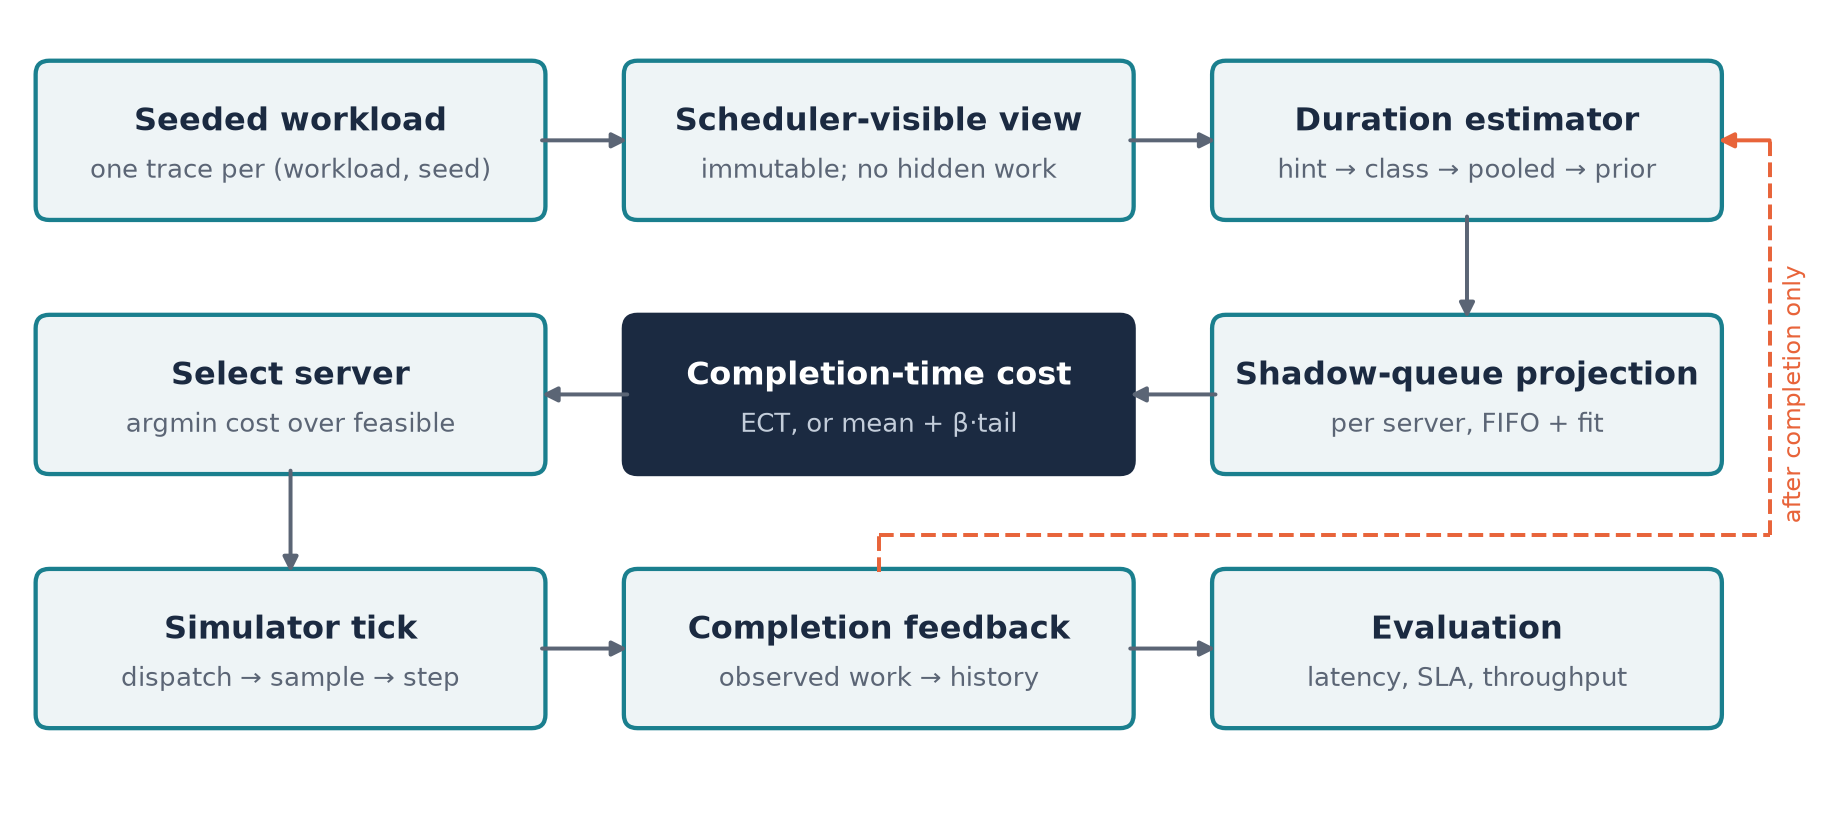
\includegraphics[width=\linewidth]{fig_architecture.png}
\caption{Decision flow for the completion-time policies. Completed tasks update the duration history only
after they finish, so a task never informs its own estimate.}\label{fig:arch}
\end{figure}

\subsection{Tick and control flow}
The simulator is time-stepped, with one tick equal to one second. Each tick (i)~dispatches the tasks
arriving at that tick, one at a time, through the policy; (ii)~samples every server's metrics into its log
and rolling window; and (iii)~advances every server, finishing tasks, releasing their resources and starting
queued tasks whose resources now fit. Sampling happens before the step, so a task that starts and finishes
within one tick still appears in utilisation. After arrivals stop, the simulator keeps stepping until every
queue is empty; a hard cutoff would silently drop the slowest tasks and flatter the policies that cause them.

\subsection{Online learning and decision}
The V2 policies learn online. When a task completes, the simulator reports its observed service time to the
policy, which converts it back to speed-1 work and stores it in a bounded history (200 samples per class).
At decision time the policy combines that history with the visible state to predict completion on every
feasible server. No parameter is fitted on test traces: the only state carried between decisions is the
history of completed tasks within the current run.

% ================================================================ 5
\section{Methodology}

\subsection{Baseline policies}
\begin{table}[H]
\caption{Policies compared.}\label{tab:policies}
\begin{tabularx}{\linewidth}{lY}
\toprule
\textbf{Policy} & \textbf{Rule}\\
\midrule
Round Robin & Cyclic order $0,1,\dots,N-1$.\\
Random & Uniform over servers (seeded stream).\\
Weighted RR & Smooth weighted round robin~\cite{nginx} with weights cores $\times$ speed.\\
Power of Two (P2C) & Sample two distinct servers, keep the lower load score $L_i$ (seeded stream).\\
Least CPU & Lowest live CPU load.\\
Weighted metric & Lowest $L_i$; the V1 policy without its risk term (V1 ablation).\\
\textbf{Probabilistic (V1)} & Lowest $S_i$ among servers with $\prisk \le 0.5$ (Section~\ref{sec:v1}).\\
\textbf{ECT-only (V2)} & Lowest predicted completion time (Section~\ref{sec:ect}).\\
\textbf{Uncertainty ECT (V2)} & Lowest mean $+\,\beta\,\times$ tail of predicted completion time (Section~\ref{sec:uect}).\\
\bottomrule
\end{tabularx}
\end{table}
Every policy subclasses one interface and only \emph{reads} state; a contract test compares the complete
server state before and after each call.

\subsection{V1: probabilistic overload-risk policy}\label{sec:v1}
For each server the balancer keeps the last $W=10$ samples of CPU load $C_i$ and memory load $M_i$ and
computes their mean and population standard deviation. With thresholds $\theta_C=80\%$ and
$\theta_M=85\%$, the exceedance probabilities under a normal approximation are
\begin{equation}
  P_C = 1-\Phi\!\left(\frac{\theta_C-\mu_C}{\sigma_C}\right),\qquad
  P_M = 1-\Phi\!\left(\frac{\theta_M-\mu_M}{\sigma_M}\right),
\end{equation}
where $\Phi$ is the standard normal CDF. If $\sigma=0$ the probability is deterministic: 1 if
$\mu>\theta$, otherwise 0. Treating the two exceedances as independent, the combined risk is
\begin{equation}
  \prisk = 1-(1-P_C)(1-P_M).
\end{equation}
With a normalised recent response time $r_i$, the load score and the risk-adjusted score are
\begin{align}
  L_i &= 0.4\,\frac{C_i}{100} + 0.4\,\frac{M_i}{100} + 0.2\,r_i, \\
  S_i &= 0.6\,L_i + 0.4\,\prisk .
\end{align}
Servers with $\prisk>0.5$ are excluded when at least one server is at or below that level. If none is, the
policy chooses the lowest $S_i$ among all servers and records the decision as \emph{capacity pressure}.
With weights $(1,0)$ and no admission filter the policy is exactly the weighted-metric baseline, and a unit test
confirms the two make identical decisions; that baseline is therefore the V1 ablation.

\subsection{Observing queued load}\label{sec:backlog}
In early runs every load-aware policy lost to load-blind Weighted RR. The cause was fragmentation: the
2-core server had 424 queued tasks yet reported only about 62\% CPU, because the task at the head of its
queue could not fit beside the one already running. The fix changed the observed signal, not the formulas:
load is (running $+$ queued demand) $\div$ capacity, which equals utilisation when there is no queue.
Least CPU's stable mean response fell from 907\,s to 6.5\,s. This signal is used by every load-aware policy
in both stages.

\subsection{V2: duration estimation}
The estimator predicts the work of the incoming task in speed-1 seconds, using this fallback order:
\begin{enumerate}
  \item a public duration hint supplied with the task, if any;
  \item the mean of completed tasks of the same visible class;
  \item the mean of all completed tasks;
  \item a global prior equal to the nominal mean work, 6\,s.
\end{enumerate}
The estimate is \emph{prequential}: a task can only influence the estimates of tasks dispatched after it has
completed. For running tasks, remaining work is estimated conservatively as the expected total minus the
work already processed, with a floor of one tick of progress, so a running task is never assumed finished.
On the stable and bursty workloads tasks carry no class or hint, so the estimator relies on pooled history
and the prior.

\subsection{V2: shadow-queue projection}\label{sec:shadow}
For each candidate server the policy builds a temporary copy of the server's running tasks and FIFO queue,
appends the incoming task, and advances the copy tick by tick using the simulator's own rules
(Algorithm~\ref{alg:shadow}): running tasks progress by the server speed, finished tasks release CPU and
memory, and the head of the queue starts only when both of its resources fit. This preserves head-of-line
blocking, which a simple ``queue length'' signal ignores. The copy is discarded after the prediction; the
real server is never modified. A server on which the task can never fit is marked infeasible.

\begin{algorithm}[H]
\caption{Shadow-queue completion-time prediction for one server}\label{alg:shadow}
\begin{algorithmic}[1]
\Require server view (running tasks, FIFO queue, $c$, $m$, speed $v$); candidate task $\tau$; predicted work $\hat w$; current tick $t$
\If{$\tau$ cannot fit on an empty server} \Return infeasible \EndIf
\State $R \gets$ running tasks with estimated remaining work; $Q \gets$ queued tasks with estimated work
\State append $\tau$ with work $\hat w$ to $Q$
\State \Call{StartFitting}{$t$}
\For{$k = t, t+1, \dots$}
  \State reduce the remaining work of every task in $R$ by $v$; remove and release finished tasks
  \If{$\tau$ finished} \Return $\widehat{\mathrm{ECT}} = (k+1) - a_\tau$ \EndIf
  \State \Call{StartFitting}{$k+1$}
\EndFor
\Statex
\Procedure{StartFitting}{$k$} \Comment{strict FIFO: stop at the first head that does not fit}
  \While{$Q \ne \emptyset$ and head of $Q$ fits in the free CPU and memory}
    \State move head of $Q$ to $R$ with start tick $k$
  \EndWhile
\EndProcedure
\end{algorithmic}
\end{algorithm}

Figure~\ref{fig:shadow} gives an illustrative example. The fast server has work ahead of the task, but its
speed still lets the task finish earlier than on the idle slow server. A least-loaded rule would prefer the
idle server.

\begin{figure}[H]
\centering
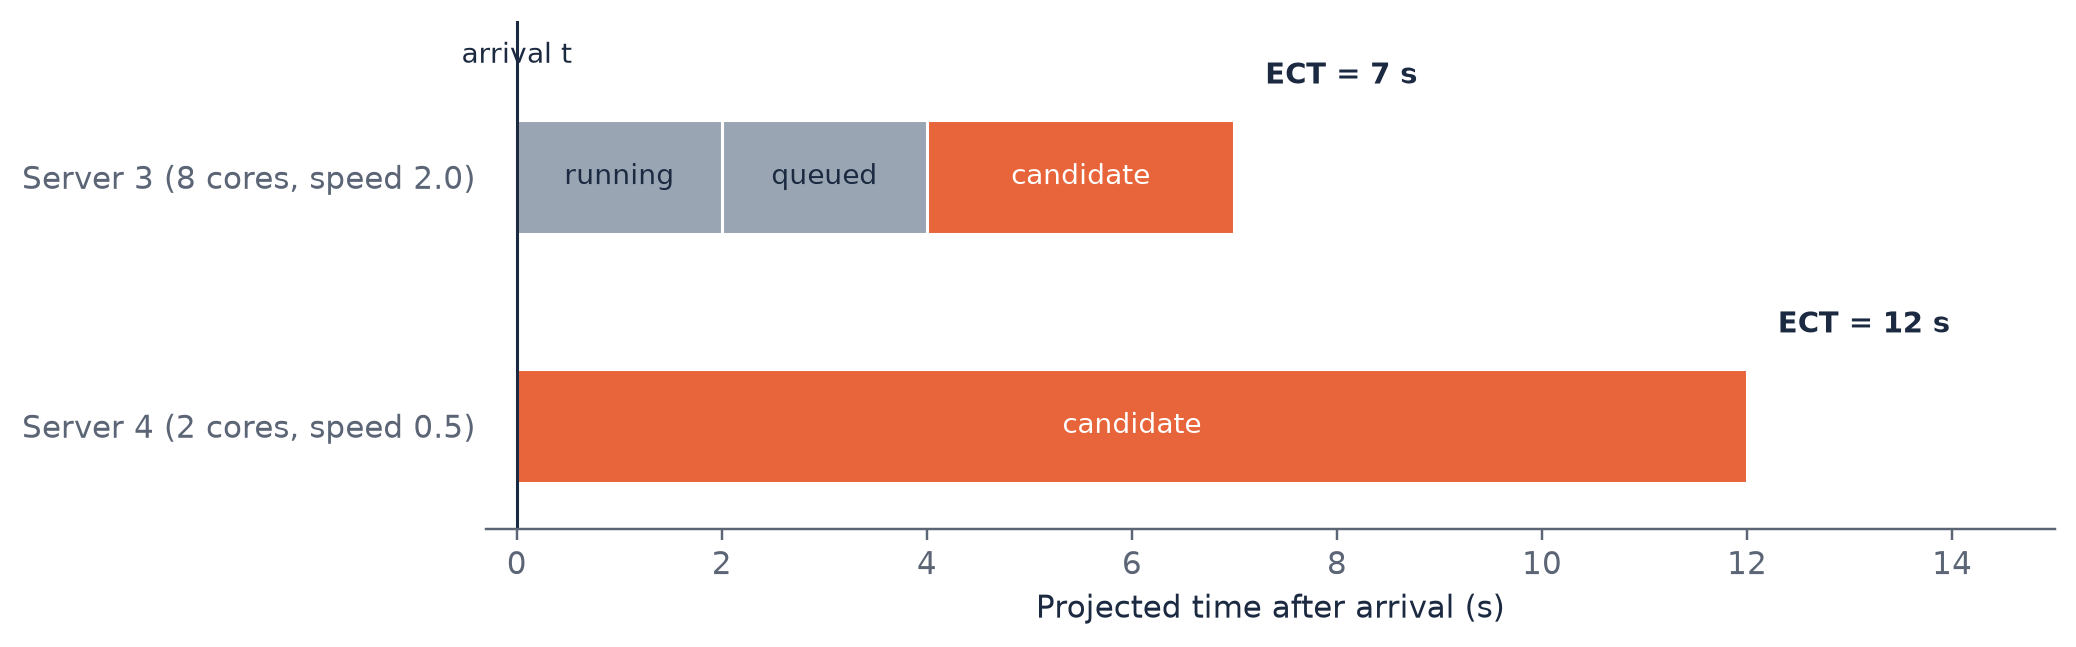
\includegraphics[width=0.92\linewidth]{fig_shadow_queue.png}
\caption{Illustrative projection for a 6\,s task (not simulation output). Queued work on the fast server
delays the start by 4\,s, but the task still finishes 5\,s earlier than on the idle slow server.}\label{fig:shadow}
\end{figure}

\subsection{V2: ECT-only policy}\label{sec:ect}
ECT-only predicts the completion time of the incoming task on every feasible server and chooses the smallest:
\begin{equation}
  i^\star = \arg\min_{i\ \mathrm{feasible}} \widehat{\mathrm{ECT}}_i, \qquad
  \widehat{\mathrm{ECT}}_i = \hat f_{\tau,i} - a_\tau ,
\end{equation}
where $\hat f_{\tau,i}$ is the projected finish tick. The prediction contains both the waiting time and the
execution time, so it accounts for queue length, head-of-line blocking, resource fit and server speed in one
quantity. Ties go to the lowest server index. Each decision costs one projection per server.

\subsection{V2: uncertainty-aware ECT}\label{sec:uect}
Instead of one work estimate, the uncertainty-aware policy runs the projection once for each value in the
duration history, giving an empirical distribution of completion times on each server. With mean
$\hat\mu_i$ and 90th percentile $\hat q_{90,i}$, its cost is
\begin{equation}
  J_i = \hat\mu_i + \beta\,\max\bigl(0,\ \hat q_{90,i}-\hat\mu_i\bigr), \qquad \beta = 0.5 .
\end{equation}
With $\beta=0$ it chooses by the mean of the distribution, close to ECT-only, so ECT-only is the matched
ablation for the uncertainty premium. A positive $\beta$ penalises servers whose completion time has a long
upper tail.

\subsection{Information boundary and oracle diagnostic}
An \emph{oracle} variant that sees each task's true work exists as a diagnostic. It is kept on a separate code
path and never enters the practical comparison. It bounds how much better duration estimates could help
under the same projection model.

% ================================================================ 6
\section{Experimental configuration}

\subsection{Experimental settings}
All tunable values live in one configuration module and were fixed before the final comparison
(Appendix~A). The main ones are mean work 6\,s; $R_{\mathrm{SLA}}=18$\,s ($3\times$ the nominal work);
target utilisation 65\%; four 50-tick bursts at $3\times$ arrivals; V1 window $W=10$, thresholds 80/85\%,
score weights 0.6/0.4 and admission level 0.5; V2 history of 200 samples and $\beta=0.5$. Randomness is passed
as explicit seeded \code{numpy.random.Generator} objects~\cite{harris2020}; randomised policies draw from their
own streams, so they cannot perturb the workload. The suite contains 159 automated tests.

\subsection{Two evaluation protocols}
The two stages were evaluated under different, separately stated protocols, and their numbers should not be
mixed.

\begin{table}[H]
\caption{Evaluation protocols.}\label{tab:protocols}
\begin{tabularx}{\linewidth}{lYY}
\toprule
 & \textbf{Protocol A (V1)} & \textbf{Protocol B (V2, matched)}\\
\midrule
Policies & 6 baselines + Probabilistic & 6 baselines + Probabilistic + ECT-only + Uncertainty ECT\\
Trace & full trace, about 3,500--4,100 tasks & first 1,000 tasks of the same traces\\
Arrival window covered & 1000\,s, all four bursts & about the first 210--250\,s; exactly one burst\\
Seeds, workloads & 0--4; stable, bursty & 0--4; stable, bursty\\
Runs & $7\times2\times5 = 70$ & $9\times2\times5 = 90$\\
Decisive comparison & Probabilistic vs.\ weighted metric & Uncertainty ECT vs.\ ECT-only; ECT vs.\ baselines\\
\bottomrule
\end{tabularx}
\end{table}

The 1,000-task cap of Protocol~B keeps the per-decision projections affordable, but it changes the workload:
each capped stable trace covers less than half of one drift period, and each capped bursty trace contains one
burst instead of four. Protocol~B results therefore describe the start of each trace, and absolute values
(for example Round Robin's mean response) are not comparable with Protocol~A.

% ================================================================ 7
\section{Evaluation protocol and performance measures}

\subsection{Metrics}
\begin{table}[H]
\caption{Performance measures.}\label{tab:metrics}
\begin{tabularx}{\linewidth}{lYc}
\toprule
\textbf{Metric} & \textbf{Definition} & \textbf{Better}\\
\midrule
Mean / p95 response & Finish $-$ arrival over completed tasks, queueing included & lower\\
SLA violation rate & Fraction of completed tasks with response $>18$\,s & lower\\
Throughput & Completed tasks $\div$ total simulated ticks, drain included & higher\\
Goodput & Tasks within the SLA $\div$ the 1000-tick arrival horizon & higher\\
CPU / memory utilisation & Mean true utilisation over the arrival horizon & context\\
Load imbalance & Mean standard deviation of CPU utilisation across servers & context\\
Overload frequency (V1) & Fraction of server-intervals above $\theta$ & lower\\
Calibration (V1) & Mean chosen $\prisk$ vs.\ observed overload frequency & diagnostic\\
Capacity pressure (V1) & Fraction of decisions in which every server had $\prisk>0.5$ & diagnostic\\
\bottomrule
\end{tabularx}
\end{table}

Because Protocol~B traces stop arriving after roughly 250\,s while goodput is divided by the full 1000-tick
horizon, its goodput values are useful only for comparing policies with each other. Imbalance is reported for
context only: on servers of different speeds, equal utilisation does not mean equal service.

\subsection{Paired comparison}
Matched seeds share a task trace, so the per-seed difference between a policy and its ablation cancels most
workload noise. The report gives the mean difference, its standard deviation and the number of seeds on which
the proposed component won. With five seeds, a 5/5 or 0/5 outcome has a one-sided sign-test $p=1/32\approx0.03$.
Confidence intervals were not used, because with $n=5$ they are wide and rely on a normality assumption.

% ================================================================ 8
\section{Results}

\subsection{V1: does the overload probability help? (Protocol A)}
Table~\ref{tab:v1main} summarises the 70 Protocol~A runs.

\begin{table}[H]
\caption{Protocol A results, mean $\pm$ standard deviation over five seeds.}\label{tab:v1main}
\centering
\small
\begin{tabular}{lrrrrrr}
\toprule
& \multicolumn{3}{c}{\textbf{Stable}} & \multicolumn{3}{c}{\textbf{Bursty}}\\
\cmidrule(lr){2-4}\cmidrule(lr){5-7}
\textbf{Policy} & Resp.\ (s) & SLA viol. & Thr.\ (/s) & Resp.\ (s) & SLA viol. & Thr.\ (/s)\\
\midrule
Round Robin     & $857 \pm 30$   & 59.2\% & 0.49 & $821 \pm 25$  & 60.0\% & 0.46\\
Random          & $847 \pm 40$   & 58.7\% & 0.50 & $823 \pm 35$  & 59.2\% & 0.46\\
Weighted RR     & $9.1 \pm 1.7$  & 7.4\%  & 3.51 & $30.9 \pm 5.2$ & 57.8\% & 3.20\\
P2C             & $24.8 \pm 4.2$ & 28.2\% & 3.26 & $46.4 \pm 7.3$ & 58.2\% & 2.76\\
Least CPU       & $6.16 \pm 0.61$ & 2.9\% & 3.94 & $29.2 \pm 4.8$ & 54.1\% & 3.43\\
Weighted metric & $\mathbf{6.15 \pm 0.62}$ & \textbf{2.7\%} & 3.95 & $29.3 \pm 4.9$ & \textbf{53.5\%} & 3.41\\
Probabilistic   & $6.44 \pm 0.74$ & 3.4\% & 3.93 & $29.5 \pm 5.2$ & 53.9\% & 3.41\\
\bottomrule
\end{tabular}
\end{table}

Load-blind policies collapse because they give the 2-core, 0.5-speed server one fifth of all tasks.
Weighted RR is competitive on the stable workload but cannot react to a burst. P2C is weak at $N=5$: a
two-server sample misses the fastest server 60\% of the time. Under bursts every policy violates the SLA for
more than half of all tasks, because offered load reaches about 160\% of capacity.

\begin{table}[H]
\caption{Paired difference $\Delta$ = probabilistic $-$ weighted metric (Protocol A). Negative is better
for the probabilistic policy, except for throughput.}\label{tab:v1paired}
\centering
\begin{tabular}{llrc}
\toprule
\textbf{Workload} & \textbf{Metric} & \textbf{$\Delta$ (mean $\pm$ std)} & \textbf{Seeds won}\\
\midrule
\multirow{3}{*}{Stable} & Mean response & $+0.29 \pm 0.25$\,s & 0/5\\
 & SLA violation rate & $+0.69 \pm 0.52$\,pp & 0/5\\
 & Overload (utilisation) & $+1.21 \pm 0.83$\,pp & 0/5\\
\midrule
\multirow{3}{*}{Bursty} & Mean response & $+0.18 \pm 0.85$\,s & 3/5\\
 & SLA violation rate & $+0.45 \pm 1.82$\,pp & 2/5\\
 & Overload (utilisation) & $-1.06 \pm 1.52$\,pp & 4/5\\
\bottomrule
\end{tabular}
\end{table}

\begin{figure}[H]
\centering
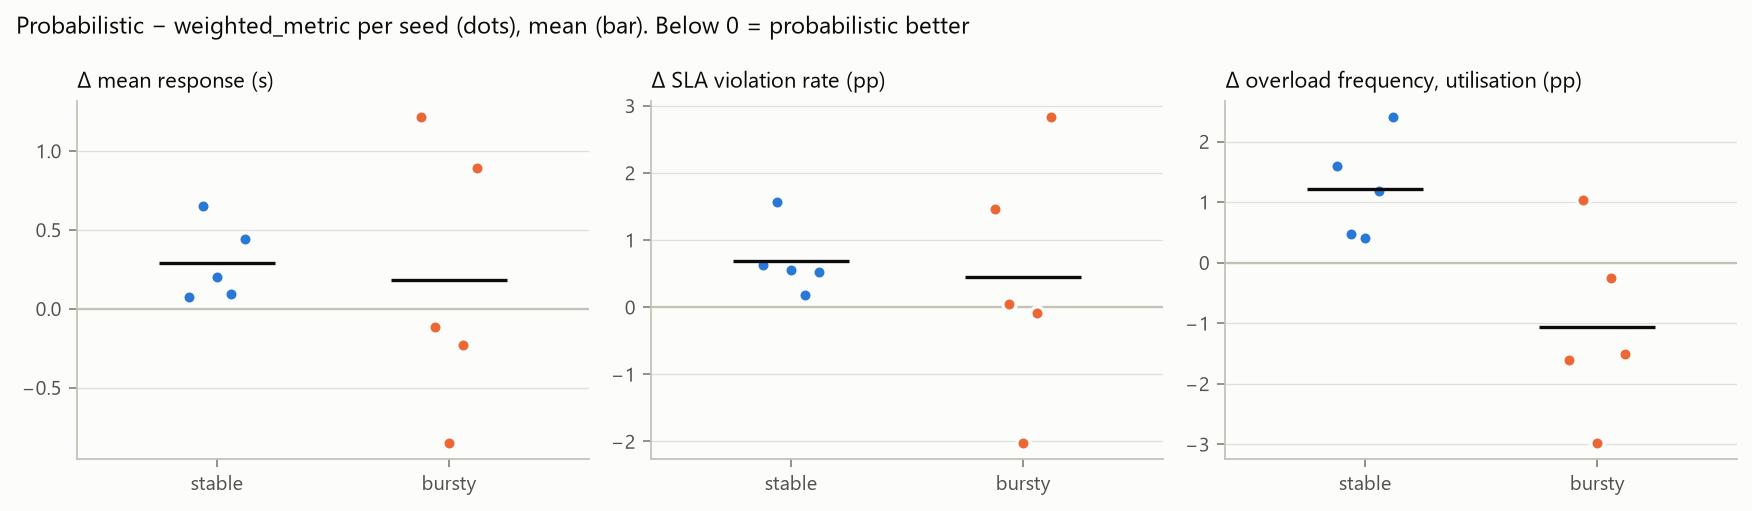
\includegraphics[width=\linewidth]{fig2_paired_by_seed.png}
\caption{Protocol A: per-seed paired differences (dots) and their mean (bar). Below zero means the risk term
helped.}\label{fig:v1paired}
\end{figure}

The pre-declared primary outcome, fewer SLA violations under bursts than the ablation, is not met. On the
stable workload the risk term is slightly but consistently harmful (0/5 seeds); under bursts every difference
lies inside the seed-to-seed noise.

\paragraph{Why: calibrated but not discriminative.} The mean $\prisk$ of the chosen server matches the
observed overload frequency closely: 0.62 vs.\ 0.62 on the stable workload and 0.74 vs.\ 0.72 under bursts
(Figure~\ref{fig:calibration}). The estimate is not wrong; it is uninformative for ranking. A load-aware
balancer equalises the servers, so their loads rise and fall together (Figure~\ref{fig:timeseries}). During a
burst all five reach 10--20$\times$ capacity at once, every server has $\prisk\approx1$, and the decision falls
back to capacity pressure. This happened in 57\% of stable and 73\% of bursty decisions. In that state $S_i$
ranks servers exactly as $L_i$ does.

\begin{figure}[H]
\centering
\begin{minipage}{0.40\linewidth}
\centering
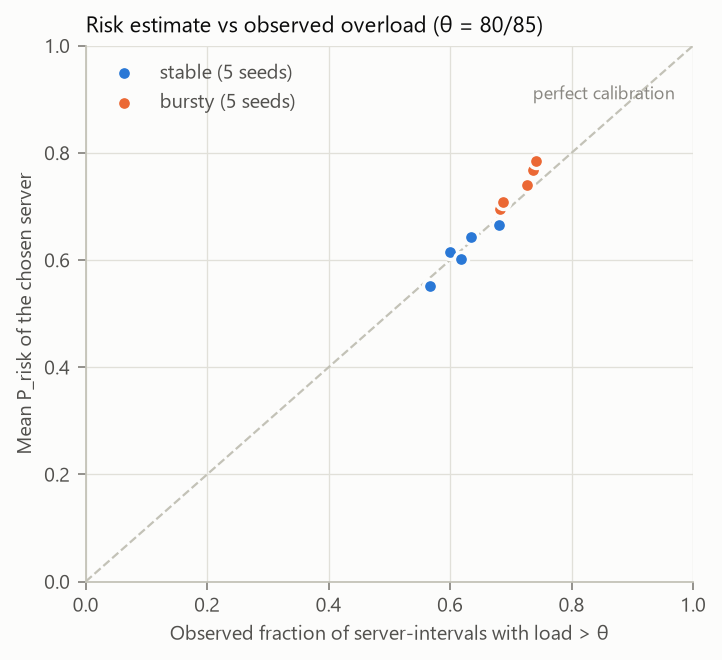
\includegraphics[width=\linewidth]{fig3_calibration.png}
\caption{Calibration of $\prisk$, one point per seed.}\label{fig:calibration}
\end{minipage}\hfill
\begin{minipage}{0.57\linewidth}
\centering
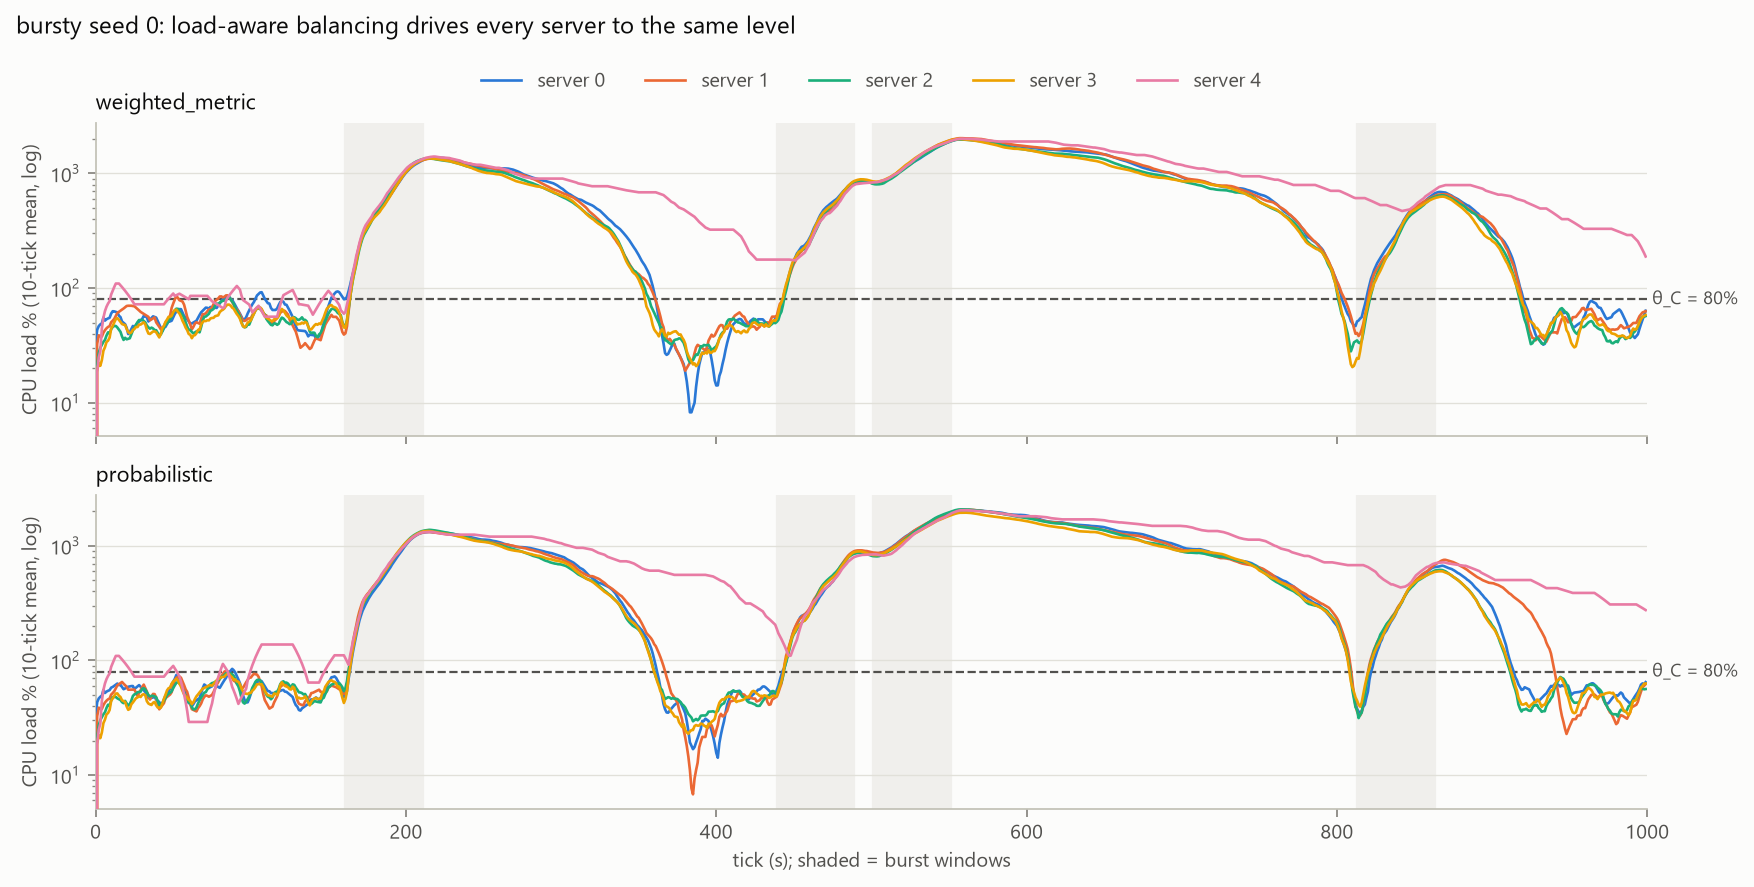
\includegraphics[width=\linewidth]{fig4_load_timeseries.png}
\caption{Bursty workload, seed 0: all servers rise together during bursts (shaded).}\label{fig:timeseries}
\end{minipage}
\end{figure}

\paragraph{Sensitivity.} Four axes were declared in advance and swept one at a time, plus a threshold
$\times$ admission grid: 44 configurations, each on both workloads and five seeds, with the ablation rerun at
every point and outcomes always scored at the frozen thresholds (Figure~\ref{fig:sensitivity}). Raising
$\theta$ to 150 cut stable capacity pressure from 57\% to 10\% without producing a consistent win; bursty
pressure stayed at 67--80\% for every $\theta$. The only consistent gain (about 1\%, 5/5 stable seeds) came
from disabling the admission filter, and the stable result grew steadily worse as the risk weight increased.
Every setting that helped did so by \emph{weakening} the risk machinery.

\begin{figure}[H]
\centering
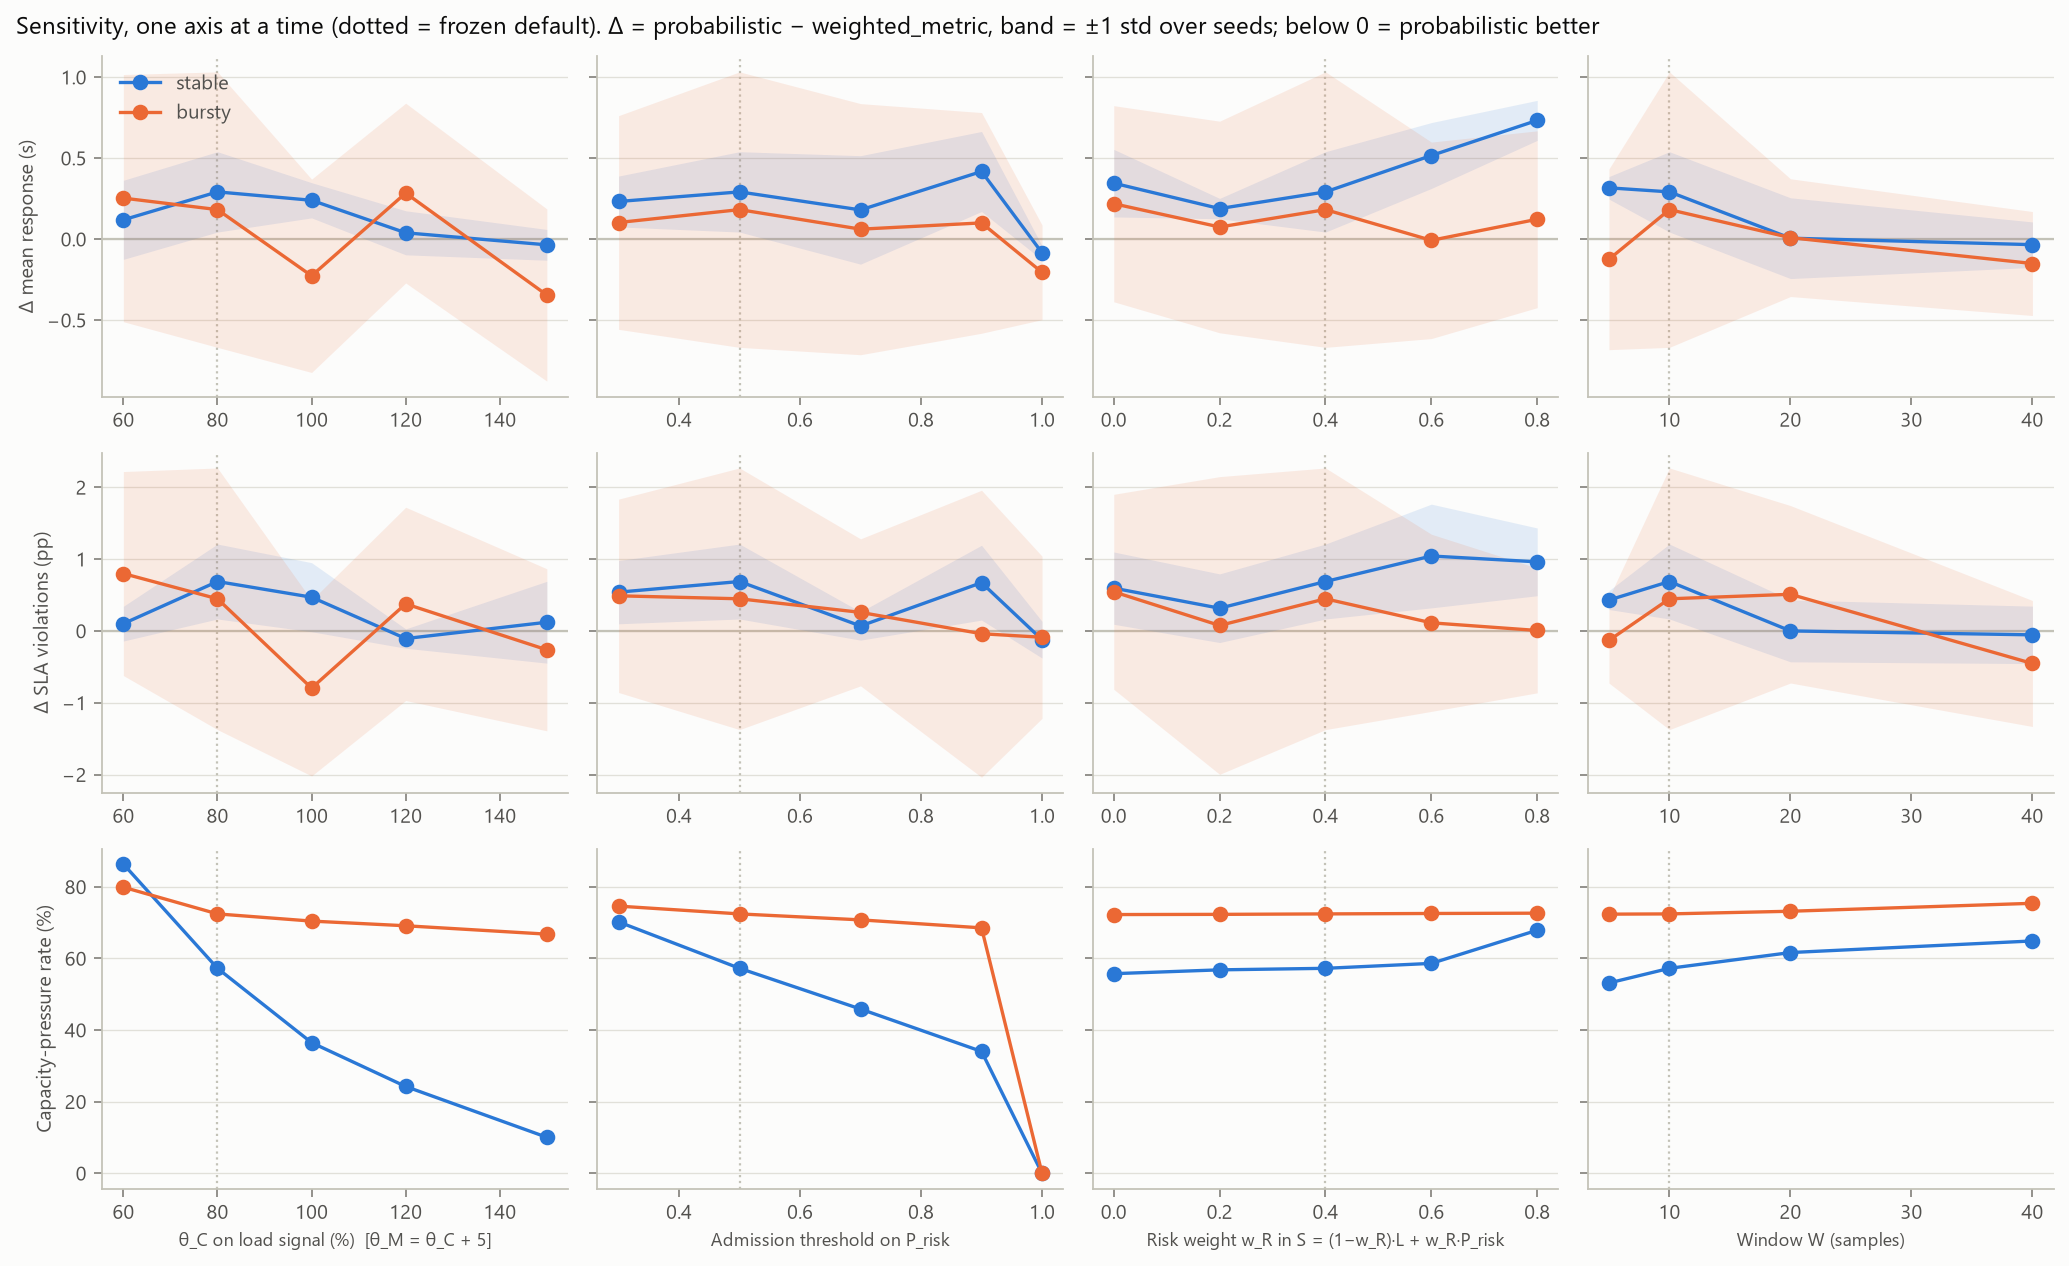
\includegraphics[width=\linewidth]{fig5_sensitivity.png}
\caption{Protocol A one-axis sensitivity. $\Delta$ = probabilistic $-$ weighted metric (band: $\pm1$ std);
bottom row: capacity-pressure rate. Dotted lines mark the frozen defaults.}\label{fig:sensitivity}
\end{figure}

\subsection{V2: completion-time prediction (Protocol B)}
Tables~\ref{tab:v2stable} and~\ref{tab:v2bursty} give the matched Protocol~B results; Figures~\ref{fig:v2resp}
and~\ref{fig:v2sla} show them graphically. Bold marks the best value in each column.

\begin{table}[H]
\caption{Protocol B, stable workload (means over five seeds; mean response $\pm$ std).}\label{tab:v2stable}
\centering
\small
\begin{tabular}{lrrrrr}
\toprule
\textbf{Policy} & \textbf{Mean resp.\ (s)} & \textbf{p95 (s)} & \textbf{SLA viol.} & \textbf{Thr.\ (/s)} & \textbf{Goodput (/s)}\\
\midrule
Round Robin        & $231.27 \pm 9.72$  & 1414.63 & 56.6\% & 0.485 & 0.434\\
Random             & $243.82 \pm 16.86$ & 1471.71 & 57.3\% & 0.474 & 0.427\\
Weighted RR        & $8.77 \pm 1.42$    & 23.80   & 8.9\%  & 3.553 & 0.911\\
P2C                & $15.64 \pm 2.91$   & 52.41   & 24.2\% & 2.765 & 0.758\\
Least CPU          & $\mathbf{6.99 \pm 1.19}$ & 16.80 & 3.9\% & 3.886 & 0.961\\
Weighted metric    & $7.11 \pm 1.23$    & 16.00   & 3.7\%  & 3.809 & 0.963\\
Probabilistic (V1) & $7.42 \pm 1.32$    & 17.40   & 4.5\%  & 4.097 & 0.955\\
\textbf{ECT-only}  & $7.70 \pm 1.39$    & \textbf{14.21} & \textbf{1.6\%} & \textbf{4.329} & \textbf{0.984}\\
Uncertainty ECT    & $9.15 \pm 1.30$    & 16.00   & 3.0\%  & 4.263 & 0.970\\
\bottomrule
\end{tabular}
\end{table}

\begin{table}[H]
\caption{Protocol B, bursty workload (means over five seeds; mean response $\pm$ std).}\label{tab:v2bursty}
\centering
\small
\begin{tabular}{lrrrrr}
\toprule
\textbf{Policy} & \textbf{Mean resp.\ (s)} & \textbf{p95 (s)} & \textbf{SLA viol.} & \textbf{Thr.\ (/s)} & \textbf{Goodput (/s)}\\
\midrule
Round Robin        & $256.44 \pm 23.56$ & 1536.55 & \textbf{56.6\%} & 0.455 & \textbf{0.434}\\
Random             & $273.73 \pm 14.12$ & 1628.88 & 56.8\% & 0.440 & 0.432\\
Weighted RR        & $32.85 \pm 4.97$   & 71.22   & 64.3\% & 3.260 & 0.357\\
P2C                & $37.53 \pm 6.08$   & 101.60  & 58.7\% & 2.097 & 0.413\\
Least CPU          & $32.70 \pm 4.41$   & 81.83   & 61.5\% & 2.609 & 0.385\\
Weighted metric    & $32.87 \pm 4.38$   & 87.03   & 60.9\% & 2.830 & 0.391\\
Probabilistic (V1) & $32.84 \pm 3.75$   & 90.21   & 62.0\% & 2.671 & 0.380\\
\textbf{ECT-only}  & $\mathbf{30.79 \pm 4.57}$ & \textbf{67.41} & 62.5\% & 3.607 & 0.375\\
Uncertainty ECT    & $31.59 \pm 4.42$   & 68.01   & 63.2\% & \textbf{3.628} & 0.368\\
\bottomrule
\end{tabular}
\end{table}

\begin{figure}[H]
\centering
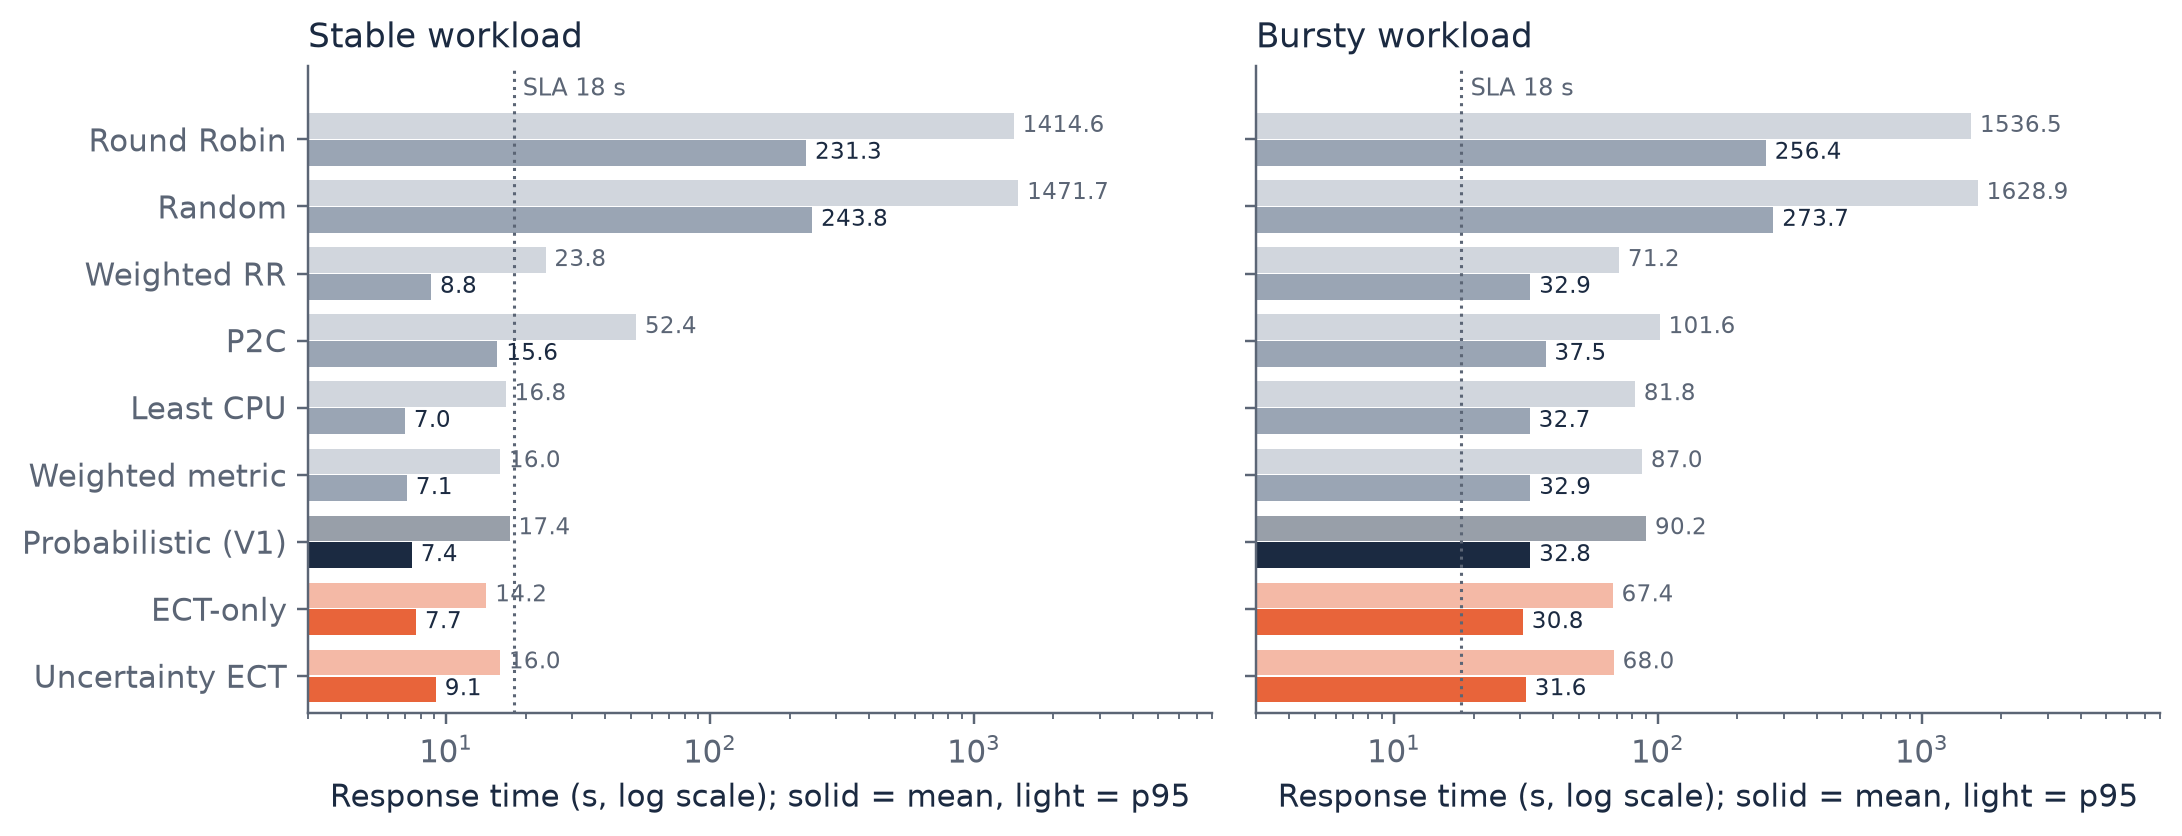
\includegraphics[width=\linewidth]{fig_v2_response.png}
\caption{Protocol B: mean (solid) and p95 (light) response time per policy, log scale. Orange marks the V2
policies. The dotted line is the 18\,s SLA.}\label{fig:v2resp}
\end{figure}

\begin{figure}[H]
\centering
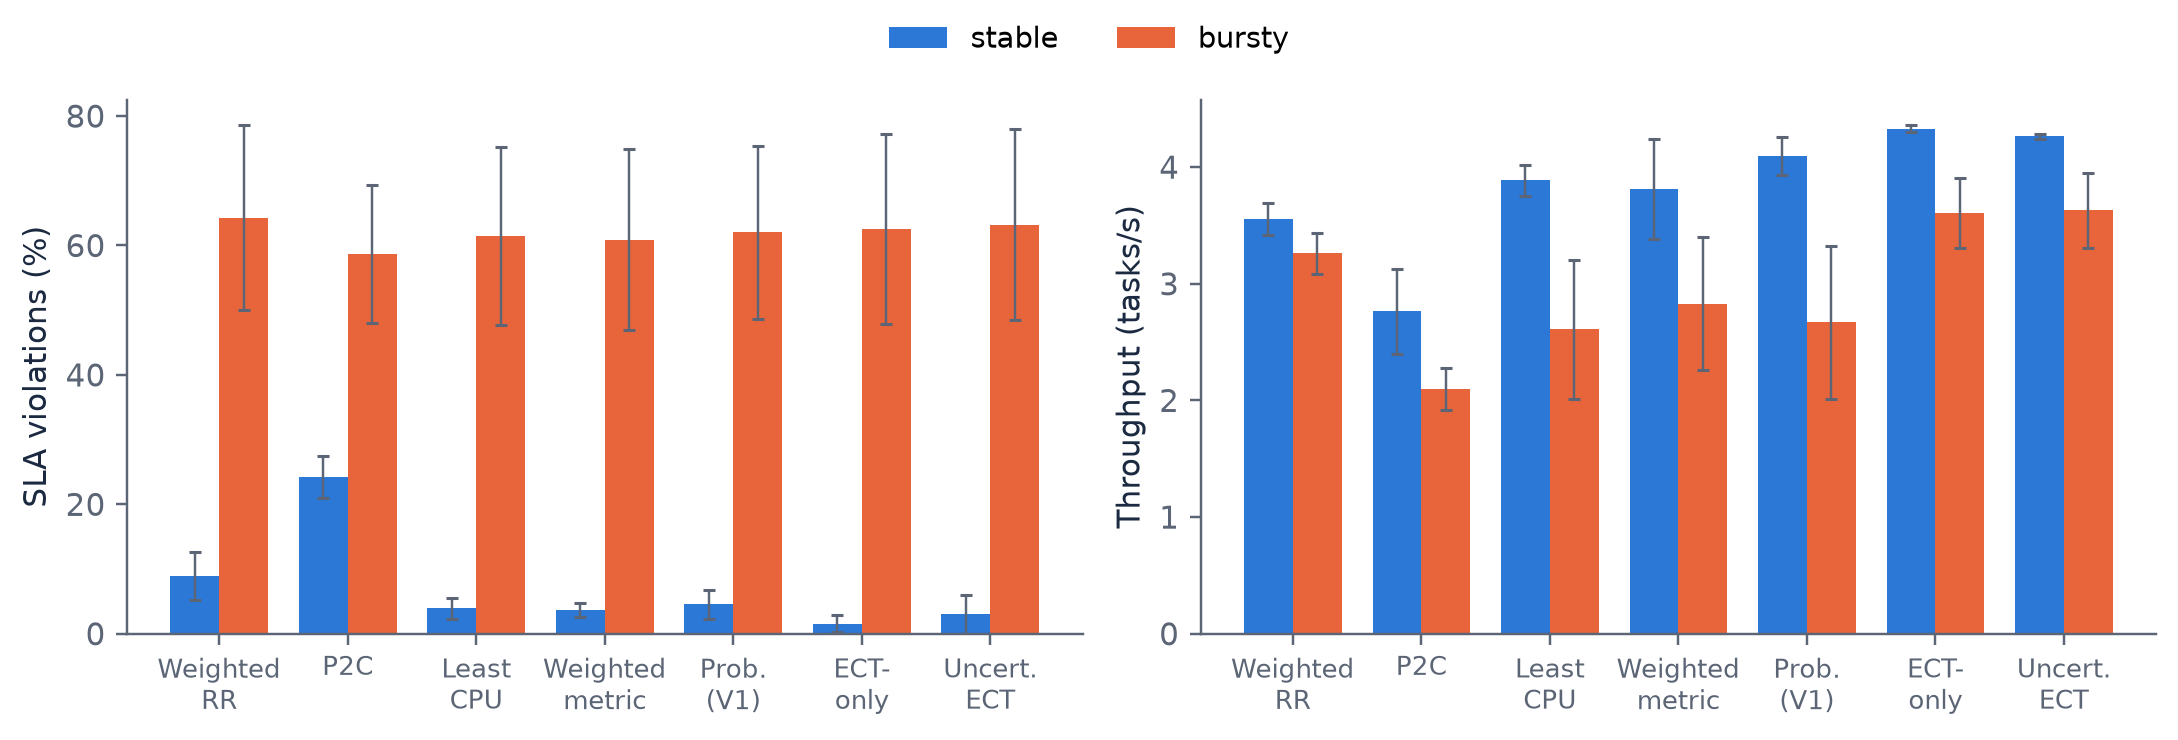
\includegraphics[width=\linewidth]{fig_v2_sla_throughput.png}
\caption{Protocol B: SLA violation rate and throughput for the load-aware policies (error bars: $\pm1$ std
over seeds).}\label{fig:v2sla}
\end{figure}

\paragraph{Stable workload.} ECT-only gives the lowest p95 (14.21\,s against 16.00\,s for the best baseline),
less than half the SLA violations of the best baseline (1.6\% vs.\ 3.7\%), and the highest throughput and
goodput. Its \emph{mean} response (7.70\,s) is slightly higher than Least CPU (6.99\,s) and the weighted metric
(7.11\,s). The pattern is consistent with a policy that prices speed explicitly: it sends more work to the
fast servers, accepting short waits there, which trims the long tail but costs a little on average. Its much
higher load imbalance (36.5 vs.\ 14.6 for Least CPU; Appendix~A) is the visible sign of that concentration.

\paragraph{Bursty workload.} ECT-only has the lowest mean (30.79\,s) and p95 (67.41\,s) of all practical
policies and about 28\% higher throughput than the weighted metric. Its SLA violation rate (62.5\%) is not the
lowest: once a burst offers more work than the cluster can process, most tasks exceed 18\,s under every
load-aware policy, and placement only changes \emph{how far} they exceed it. Round Robin's lower violation rate
is an artefact of its pathology: tasks sent to the four fast servers finish quickly while those sent to
server~4 wait for hundreds of seconds, as its 1536\,s p95 shows.

\paragraph{Paired comparison with the strongest baselines.} Averages can hide seed-to-seed variation, so
Table~\ref{tab:v2vsbase} compares ECT-only with the two strongest load-aware baselines seed by seed. The
pattern is clear-cut: ECT-only wins on all five seeds for stable p95, stable SLA violations, throughput on both
workloads, and bursty mean and p95 response, and it loses on all five seeds for stable mean response. The bursty
SLA difference is within seed noise.

\begin{table}[H]
\caption{Paired difference = ECT-only $-$ baseline (Protocol B), mean $\pm$ std over five seeds, with the
number of seeds on which ECT-only was better. Negative is better for ECT-only, except for throughput.}\label{tab:v2vsbase}
\centering
\small
\begin{tabular}{llrcrc}
\toprule
& & \multicolumn{2}{c}{\textbf{vs.\ Least CPU}} & \multicolumn{2}{c}{\textbf{vs.\ Weighted metric}}\\
\cmidrule(lr){3-4}\cmidrule(lr){5-6}
\textbf{Workload} & \textbf{Metric} & \textbf{Difference} & \textbf{Won} & \textbf{Difference} & \textbf{Won}\\
\midrule
\multirow{4}{*}{Stable} & Mean response & $+0.71 \pm 0.22$\,s & 0/5 & $+0.59 \pm 0.23$\,s & 0/5\\
 & p95 response & $-2.59 \pm 0.88$\,s & 5/5 & $-1.79 \pm 0.44$\,s & 5/5\\
 & SLA violation rate & $-2.34 \pm 0.51$\,pp & 5/5 & $-2.14 \pm 0.37$\,pp & 5/5\\
 & Throughput & $+0.44 \pm 0.11$\,/s & 5/5 & $+0.52 \pm 0.42$\,/s & 5/5\\
\midrule
\multirow{4}{*}{Bursty} & Mean response & $-1.91 \pm 0.60$\,s & 5/5 & $-2.09 \pm 0.76$\,s & 5/5\\
 & p95 response & $-14.42 \pm 3.36$\,s & 5/5 & $-19.62 \pm 5.41$\,s & 5/5\\
 & SLA violation rate & $+1.00 \pm 2.05$\,pp & 1/5 & $+1.60 \pm 1.98$\,pp & 1/5\\
 & Throughput & $+1.00 \pm 0.45$\,/s & 5/5 & $+0.78 \pm 0.35$\,/s & 5/5\\
\bottomrule
\end{tabular}
\end{table}

\subsection{Uncertainty premium ablation}
The uncertainty-aware policy and ECT-only share the estimator and the projection; only the premium differs.

\begin{table}[H]
\caption{Paired difference = uncertainty ECT $-$ ECT-only (Protocol B). Negative is better for the
uncertainty premium, except for throughput.}\label{tab:v2paired}
\centering
\begin{tabular}{llrc}
\toprule
\textbf{Workload} & \textbf{Metric} & \textbf{Mean difference} & \textbf{Seeds won by premium}\\
\midrule
\multirow{4}{*}{Stable} & Mean response & $+1.454$\,s & 0/5\\
 & p95 response & $+1.790$\,s & 0/5\\
 & SLA violation rate & $+1.42$\,pp & 0/5\\
 & Throughput & $-0.0665$\,/s & 0/5 (1 tie)\\
\midrule
\multirow{4}{*}{Bursty} & Mean response & $+0.807$\,s & 0/5\\
 & p95 response & $+0.600$\,s & 0/5 (2 ties)\\
 & SLA violation rate & $+0.72$\,pp & 0/5\\
 & Throughput & $+0.0217$\,/s & 3/5\\
\bottomrule
\end{tabular}
\end{table}

\begin{figure}[H]
\centering
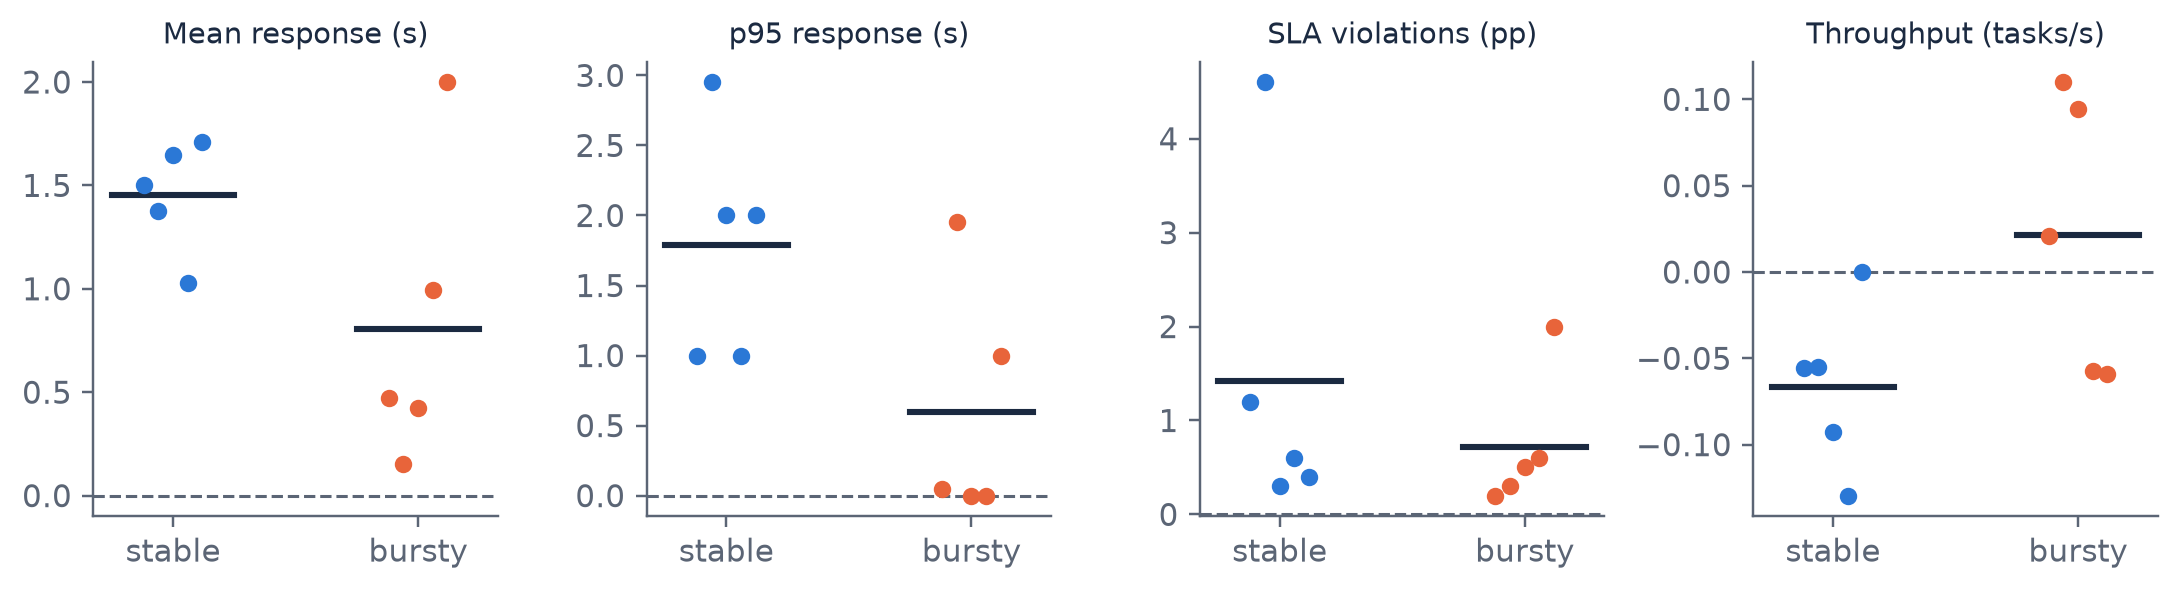
\includegraphics[width=\linewidth]{fig_v2_ablation.png}
\caption{Protocol B: per-seed paired differences, uncertainty ECT $-$ ECT-only (dots), with their mean (bar).
Below zero means the premium helped, except for throughput.}\label{fig:v2ablation}
\end{figure}

The premium made every latency and SLA measure worse on every seed of both workloads (sign test
$p\approx0.03$ per measure). Its only favourable result is a small bursty throughput gain on 3 of 5 seeds.
The mechanism mirrors the V1 finding. On these workloads tasks carry no class or hint, so the sampled
durations are the pooled history of all tasks, and the only quantity that varies across the samples is the
incoming task's own work. Its completion time on server $i$ therefore spreads by roughly that work's spread
divided by the speed $v_i$: the \emph{same} uncertainty on every server, scaled by $1/v_i$. The premium adds
nothing server-specific; it is effectively an extra penalty on slow servers, which ECT already prices through
the mean. The policy consequently concentrates even more work on the fast servers, whose queues grow (stable
mean queue length 4.02 vs.\ 2.80 for ECT-only; Appendix~A), and the extra waiting outweighs any tail benefit.
As in V1, the uncertainty describes the workload rather than the servers, so it cannot help rank them.

% ================================================================ 9
\section{Limitations and threats to validity}

\begin{table}[H]
\caption{Major validity threats and their consequences.}\label{tab:threats}
\begin{tabularx}{\linewidth}{lYY}
\toprule
\textbf{Threat} & \textbf{Condition} & \textbf{Consequence}\\
\midrule
Truncated traces & Protocol B uses the first 1,000 tasks (about 250\,s, one burst) & V2 results describe the start of each trace; full-length behaviour is untested\\
Few seeds & Five seeds per workload & Effects below about 1\% cannot be resolved\\
Synthetic workload & Independent task draws; bursts hit every server equally & Real traces~\cite{reiss2012,tirmazi2020} have per-tenant correlation and uneven volatility\\
Uninformative task metadata & Stable and bursty tasks carry no class or hint & Duration estimates fall back to pooled history; the heterogeneous workload is untested in the matched comparison\\
Normal approximation (V1) & Skewed, autocorrelated load; only 10 samples & Tail risk is crude during transitions\\
Independence (V1) & Queue couples CPU and memory & Joint risk is overstated\\
Fresh telemetry & The scheduler sees the exact current state & Stale or sampled metrics, as in production, are untested\\
Single dispatcher & One decision at a time & Herding between concurrent dispatchers is absent\\
Tick discretisation & Run times rounded up to whole ticks & Absolute times are slightly pessimistic; identical for all policies\\
Hand-set parameters & Weights, $\beta$ and thresholds fixed by design & Not jointly optimised; V2 has no sensitivity sweep\\
\bottomrule
\end{tabularx}
\end{table}

The most important limitation is the first. V1 was evaluated on complete traces with a sensitivity sweep; V2 has
so far been evaluated only on truncated traces at one parameter setting. The V2 conclusions are therefore
promising but less established than the V1 conclusions.

% ================================================================ 10
\section{Recommended research and engineering plan}

\subsection{Strengthen the V2 evaluation}
Run the V2 matrix on complete traces with all four bursts, extend to 30--50 held-out seeds, and report paired
differences of ECT-only against the strongest baseline on each metric. Evaluate the heterogeneous workload,
where class history and duration hints give the estimator real information, and add the oracle as an upper
bound so that the cost of estimation error can be measured directly. Sweep $\beta$ and the history size on
separate validation seeds before any test-seed comparison.

\subsection{Test the conditions where uncertainty should matter}
Both stages predict the same regime for uncertainty to help: servers that \emph{differ} in volatility at similar
load, and telemetry that is stale or sampled every 15--60\,s, so that variance expresses uncertainty about the
present state. Experiments with per-server background load, noisy duration hints and delayed metrics would test
this directly. A soft risk penalty should replace the hard V1 admission filter, which was the component that
hurt most.

\subsection{Path to a real deployment}
Node exporters already publish CPU, memory and queue depth to systems such as Prometheus. A scheduler sidecar
could maintain the duration history and shadow projections and expose the result as a backend weight for a
request balancer, or as a score plugin in the Kubernetes scheduling framework~\cite{k8sframework}, where
feasibility maps to a filter plugin. The projection costs one short simulation per server per decision; at
larger scale it would need a cap on projection depth or an analytic approximation.

\begin{table}[H]
\caption{Suggested milestones and the evidence each requires.}\label{tab:milestones}
\begin{tabularx}{\linewidth}{lY}
\toprule
\textbf{Milestone} & \textbf{Evidence needed before claiming completion}\\
\midrule
Full-length V2 evaluation & All four bursts; paired ECT vs.\ best baseline over $\ge 30$ seeds\\
Informative metadata & Heterogeneous workload results, with oracle upper bound\\
Robustness & Stale telemetry, noisy hints, per-server background volatility\\
Parameter study & $\beta$ and history size tuned on validation seeds only\\
Deployment prototype & Measured decision latency; behaviour with concurrent dispatchers\\
\bottomrule
\end{tabularx}
\end{table}

% ================================================================ 11
\section{Conclusion}
This project built a reproducible simulator for task placement on heterogeneous cloud servers and used it to
test two ways of making a load balancer anticipate rather than react.

The first, a variance-based overload probability, did not beat its own ablation at the declared parameters or
anywhere in a 44-point sensitivity sweep. Its estimates were calibrated but not discriminative: a good
load-aware balancer makes servers move together, so a per-server risk score has nothing to rank. The same
stage found that observing queued demand, not just utilisation, is the dominant factor, worth about two orders
of magnitude in response time.

The second, task-level completion-time prediction through a shadow copy of each server's queue, gave the best
p95 latency on both workloads, the fewest stable SLA violations, the highest stable throughput and the lowest
bursty mean response in a matched five-seed evaluation of truncated traces. It did not give the best stable mean
response. An uncertainty premium on the predicted tail made ECT worse on every latency and SLA measure.

Taken together, the results suggest that the choice of predicted quantity matters more than attaching
uncertainty to it: predicting \emph{when this task will finish here} was useful, whereas predicting
\emph{how likely this server is to be overloaded} was not. These are simulation results with the limitations
listed in Section~9; full-length traces, more seeds and realistic telemetry are needed before stronger claims
can be made.

% ================================================================ references
\phantomsection
\addcontentsline{toc}{section}{References}
\begin{thebibliography}{99}
\bibitem{dean2013} J.~Dean and L.~A. Barroso, ``The tail at scale,'' \emph{Communications of the ACM},
  vol.~56, no.~2, pp.~74--80, 2013.
\bibitem{nginx} nginx, ``Smooth weighted round-robin balancing,'' source file
  \code{src/http/ngx\_http\_upstream\_round\_robin.c}, \url{https://github.com/nginx/nginx}.
\bibitem{azar1999} Y.~Azar, A.~Z. Broder, A.~R. Karlin, and E.~Upfal, ``Balanced allocations,''
  \emph{SIAM Journal on Computing}, vol.~29, no.~1, pp.~180--200, 1999.
\bibitem{mitzenmacher2001} M.~Mitzenmacher, ``The power of two choices in randomized load balancing,''
  \emph{IEEE Transactions on Parallel and Distributed Systems}, vol.~12, no.~10, pp.~1094--1104, 2001.
\bibitem{lu2011} Y.~Lu, Q.~Xie, G.~Kliot, A.~Geller, J.~R. Larus, and A.~Greenberg, ``Join-Idle-Queue: A novel
  load balancing algorithm for dynamically scalable web services,'' \emph{Performance Evaluation}, vol.~68,
  no.~11, pp.~1056--1071, 2011.
\bibitem{verma2015} A.~Verma, L.~Pedrosa, M.~Korupolu, D.~Oppenheimer, E.~Tune, and J.~Wilkes,
  ``Large-scale cluster management at Google with Borg,'' in \emph{Proc.\ EuroSys}, 2015.
\bibitem{reiss2012} C.~Reiss, A.~Tumanov, G.~R. Ganger, R.~H. Katz, and M.~A. Kozuch, ``Heterogeneity and
  dynamicity of clouds at scale: Google trace analysis,'' in \emph{Proc.\ ACM Symposium on Cloud Computing
  (SoCC)}, 2012.
\bibitem{tirmazi2020} M.~Tirmazi, A.~Barker, N.~Deng, M.~E. Haque, Z.~G. Qin, S.~Hand, M.~Harchol-Balter, and
  J.~Wilkes, ``Borg: the next generation,'' in \emph{Proc.\ EuroSys}, 2020.
\bibitem{gneiting2007} T.~Gneiting, F.~Balabdaoui, and A.~E. Raftery, ``Probabilistic forecasts, calibration
  and sharpness,'' \emph{Journal of the Royal Statistical Society: Series B}, vol.~69, no.~2, pp.~243--268, 2007.
\bibitem{braun2001} T.~D. Braun, H.~J. Siegel, N.~Beck, \emph{et al.}, ``A comparison of eleven static heuristics
  for mapping a class of independent tasks onto heterogeneous distributed computing systems,'' \emph{Journal of
  Parallel and Distributed Computing}, vol.~61, no.~6, pp.~810--837, 2001.
\bibitem{harris2020} C.~R. Harris \emph{et al.}, ``Array programming with NumPy,'' \emph{Nature}, vol.~585,
  pp.~357--362, 2020.
\bibitem{k8sframework} Kubernetes Documentation, ``Scheduling Framework,''
  \url{https://kubernetes.io/docs/concepts/scheduling-eviction/scheduling-framework/}.
\end{thebibliography}

% ================================================================ appendices
\section*{Appendix A. Parameters and resource metrics}
\addcontentsline{toc}{section}{Appendix A. Parameters and resource metrics}

\begin{table}[H]
\caption{Frozen parameters.}\label{tab:params}
\centering
\small
\begin{tabular}{lll}
\toprule
\textbf{Parameter} & \textbf{Value} & \textbf{Note}\\
\midrule
Servers & 5 (Table~\ref{tab:servers}) & heterogeneous\\
Tick, horizon & 1\,s; arrivals for 1000\,s, then drain & \\
Task CPU, memory & $U(0.5,1.5)$ cores, $U(0.5,3)$\,GB & \\
Task work & lognormal, mean 6\,s, shape 0.6, $\ge 1$\,s & hidden from scheduler\\
Arrivals & Poisson, $\approx4$/s, $\pm20\%$ drift (period 500\,s) & $\approx65\%$ load\\
Bursts & $4\times50$\,s, $3\times$ arrivals, $1.3\times$ CPU & mean load matched\\
$R_{\mathrm{SLA}}$ & 18\,s & $3\times$ mean work\\
V1 window $W$ & 10 samples & population std\\
V1 $\theta_C$, $\theta_M$ & 80\%, 85\% & on the load signal\\
V1 weights $L$; $S$ & 0.4/0.4/0.2; 0.6/0.4 & \\
V1 admission level & 0.5 & \\
V2 duration history & 200 samples per class & prequential\\
V2 prior work & 6\,s & \\
V2 $\beta$; tail quantile & 0.5; 90th percentile & \\
Seeds & 0--4 & \\
\bottomrule
\end{tabular}
\end{table}

\begin{table}[H]
\caption{Protocol B resource metrics (means over five seeds).}\label{tab:resources}
\centering
\small
\begin{tabular}{lrrrrrr}
\toprule
& \multicolumn{3}{c}{\textbf{Stable}} & \multicolumn{3}{c}{\textbf{Bursty}}\\
\cmidrule(lr){2-4}\cmidrule(lr){5-7}
\textbf{Policy} & CPU util. & Imbalance & Queue len. & CPU util. & Imbalance & Queue len.\\
\midrule
Round Robin        & 29.7\% & 26.6 & 33.5 & 32.8\% & 28.8 & 36.0\\
Random             & 29.8\% & 27.3 & 35.2 & 32.7\% & 29.0 & 37.9\\
Weighted RR        & 63.9\% & 18.2 & 2.86 & 66.2\% & 16.0 & 18.4\\
P2C                & 56.2\% & 21.4 & 5.75 & 51.3\% & 23.1 & 13.7\\
Least CPU          & 69.7\% & 14.6 & 1.71 & 57.2\% & 18.1 & 14.8\\
Weighted metric    & 68.6\% & 14.6 & 1.75 & 61.0\% & 16.7 & 16.1\\
Probabilistic (V1) & 72.5\% & 14.9 & 2.17 & 57.6\% & 17.2 & 15.2\\
ECT-only           & 61.1\% & 36.5 & 2.80 & 65.8\% & 19.2 & 19.1\\
Uncertainty ECT    & 59.0\% & 36.9 & 4.02 & 64.7\% & 21.1 & 19.8\\
\bottomrule
\end{tabular}
\end{table}

\section*{Appendix B. Reproducing the results}
\addcontentsline{toc}{section}{Appendix B. Reproducing the results}
The code, tests, decision log and figures are at \repourl. With Python $\ge 3.11$:
\begin{verbatim}
python -m venv .venv
.venv\Scripts\Activate.ps1          # Linux/macOS: source .venv/bin/activate
pip install -r requirements.txt
pip install -e .
python -m pytest -q                  # 159 tests
python -m experiments.run_all        # Protocol A: 70 runs
python -m experiments.sensitivity    # Protocol A: 44-point sweep
python -m experiments.run_v2 --seeds 0 1 2 3 4 --workloads stable bursty \
       --limit 1000 --out results/v2  # Protocol B: 90 runs
python report/make_figures.py        # report figures -> report/figures/
\end{verbatim}

\section*{Appendix C. Key design decisions}
\addcontentsline{toc}{section}{Appendix C. Key design decisions}
\begin{table}[H]
\caption{Key design decisions (full log in \code{docs/decisions.md}).}\label{tab:decisions}
\small
\begin{tabularx}{\linewidth}{lY}
\toprule
\textbf{ID} & \textbf{Decision}\\
\midrule
D1 & Time-stepped simulator (1 tick = 1\,s) for simplicity and an exact per-tick metric log.\\
D3 & Strategy pattern: every policy implements one interface and only reads state.\\
D4 & Drain all queues at the end of a run, so the slowest tasks are not dropped.\\
D9 & Stable and bursty workloads have matched mean offered load.\\
D10 & $R_{\mathrm{SLA}} = 18$\,s fixed before any results.\\
D11 & Reservation-based servers with a strict FIFO queue.\\
D18--D19 & Utilisation hides backlog; the balancer observes load including queued demand.\\
D23 & Paired per-seed differences with win counts instead of confidence intervals.\\
D26 & Sensitivity one axis at a time plus a grid, with the ablation rerun at every point.\\
V2 & Immutable scheduler view without hidden work; prequential duration history; shadow projection that
reuses the simulator's tick rules; oracle kept on a separate path.\\
\bottomrule
\end{tabularx}
\end{table}

\end{document}
